\documentclass{beamer}

%\usepackage{subfigure}
\usepackage{graphicx}
\usepackage{sidecap}
\usepackage{caption}
\usepackage{subcaption}
\captionsetup{compatibility=false}
\usepackage{appendixnumberbeamer}
\usepackage{amsmath}
% --
\usepackage{multirow}
\usepackage{xcolor}
\usepackage{setspace}
\usepackage{hyperref}
\usepackage{anyfontsize}

\setbeamertemplate{footline}

\newenvironment{itemise} {\begin{itemize} \setlength{\itemsep}{0.2cm}} {\end{itemize}}
\usepackage[labelformat=empty]{caption}
\setbeamertemplate{sections/subsections in toc}[square]

%% COLORS
\definecolor{Gray}{gray}{0.9}
\definecolor{dblue}{rgb}{0.132,0.1,0.27}
\definecolor{mint}{cmyk}{1.0, 0.2, 0.6, 0.05}
\definecolor{ant}{cmyk}{0.5, 0.1, 0.0, 0.45}
\definecolor{lgray}{cmyk}{0.12, 0.0, 0.0, 0.17}
\definecolor{lred}{cmyk}{0.0, 0.9, 0.7, 0.0}


\usepackage{etoolbox}% http://ctan.org/pkg/etoolbox 
\usepackage{booktabs}

\newenvironment{literatur}{%
  \parskip2pt \parindent0pt \raggedright
  \def\lititem{\hangindent=0.5cm \hangafter1}}{%
  \par\ignorespaces}

\newcommand{\tb}[1]{{\color{blue}{\textbf{#1}}}}
\newcommand{\tm}[1]{{\color{mint}{\textbf{#1}}}}
\newcommand{\tr}[1]{{\color{red}{\textbf{#1}}}}
% Ilya: packages

\usepackage{tikz}
\usepackage{lmodern}
\usepackage{enumitem}

% Ilya: my commands

\newenvironment{mytemize}
{\vfill\itemize[nolistsep,itemsep=\fill,label=\color{blue}{$\triangleright$}]}
  {\enditemize}


\newenvironment{mynumerate}
{\vfill\enumerate[nolistsep,itemsep=\fill,label=\arabic*.]}
  {\endenumerate}

\newcommand{\hitem}[1]{
  {\color{blue}{$\triangleright$}} 
  {#1} 
  {\hfill}
}

\setlist[itemize]{label= \color{blue}{$\triangleright$}}
\setlist[enumerate]{label = \arabic*.}

\newcommand{\rarr}{$\Rightarrow$\ }

%------------------------------------------------------------------------------------
% TITLE
%------------------------------------------------------------------------------------
\title[PSME]{Macroeconomics\\ Lecture 10 -- Open Macroeconomy II}
\author[I. Eryzhenskiy]{Ilya Eryzhenskiy}
\institute[Paris-1]{PSME Panth\'{e}on-Sorbonne Master in Economics}
\date[PSME macro]{Fall 2022}

%---BEGIN------------------------------------------------------------------------------
\begin{document}
%---BEGIN------------------------------------------------------------------------------
\begin{frame}
\maketitle
\end{frame}
%---FRAME------------------------------------------------------------------------------
%\section{Outline}
\begin{frame}
\frametitle{Outline}
\tableofcontents
\end{frame}

\section{Balance of Payments basics}
\begin{frame}
\frametitle{Outline}
\tableofcontents[currentsection]
\end{frame}

\begin{frame}{Balance of Payments -- full picture}
  Balance of Payments is an accounting system for international transactions of an economy. The standard \tb{double entry} accounting principle applies.
  Structure: 
  \begin{mynumerate}
  \item \tb{Current account (CA)}
	\begin{mytemize}
	\item \tb{Trade Balance} a.k.a. \tb{Primary Current Account (PCA)} %: mainly Exports $-$ Imports
	\item \tb{Income Balance}
	\item Secondary income balance a.k.a. Net Unilateral Transfers
	\end{mytemize}
  \item Capital Account 
  \item \tb{Financial Account}
  \item Errors and Omissions
  \end{mynumerate}
\end{frame}

\begin{frame}{Current Account (CA): full, simplified}

Current account mainly records international \textbf{flows of goods and
services} and \textbf{incomes from factors of production}.

\begin{mytemize}
 
\item
  Flows of goods and services: \tb{Trade Balance} a.k.a. \tb{Primary
  Current Account}: exports \textbf{minus} imports of goods and
  services
\item
  Incomes from factors of production -- \tb{Income balance}:

  \begin{mynumerate}
   
   
  \item
    \underline{Capital (financial)}: Financial incomes of residents
    abroad \textbf{minus} financial incomes of non-residents in the
    economy
  \item
    \underline{Labor}: Wages of resident workers abroad \textbf{minus}
    wages of foreign workers in the economy
  \end{mynumerate}
\end{mytemize}

Secondary income balance a.k.a. net unilateral transfers -- flows of
\emph{free} goods and services -- happening without sale or purchase.
\vfill Simplifying assumptions for lecture:

\begin{mytemize}
 
\item
  Labor only supplied domestically \rarr only net financial incomes in
  the \tb{income balance}
\item
  No unilateral transfers
\end{mytemize}

\end{frame}

\begin{frame}[fragile]{%
\protect\hypertarget{capital-account}{%
Capital account}}

    \alert{Not to be confused with Financial Account (see below)!}
  \vfill
A financial analogue of unilateral transfers:
changes in asset positions that are not due to purchase/sale of assets.
\vfill Examples: debt forgiveness, assets of migrants
that change residence status. \vfill Assumed null for
rest of the course.

\end{frame}

\begin{frame}{%
\protect\hypertarget{financial-account-fa}{%
Financial Account (FA)}}

Financial account -- financial/monetary transactions underlying flows of
goods, services, and incomes. 

Equivalently, it records
changes in asset positions, or
\tb{capital flows}. \\
\vfill
Financial Account balance: change
in foreign assets of residents (\tb{capital outflows}) \textbf{minus}
change in assets of non-residents in the economy -- foreign
\textbf{liabilities} of residents (\tb{capital inflows}).
\vfill 
Sign convention (IMF): \textbf{+} for capital
outflows, \textbf{--} for capital inflows. \alert{Attenition} the sign
convention was opposite before mid-2010s! \vfill Examples: purchase of
foreign currency by household (\textbf{+} FA), increase of foreign
exchange reserves of Central bank (same), foreign direct investment
received from abroad (\textbf{--} FA) \vfill In this lecture, we study
determination of CA (real economy) and recover FA from the Balance of
Payments identity (see below).

\end{frame}

\begin{frame}{%
\protect\hypertarget{double-entry-bop-identity}{%
Double entry, BOP identity}}

Most transactions are recorded in CA and in FA \emph{{[}think of
examples of other cases{]}}. \vfill Examples of double entry:

\begin{mynumerate}
 
 
\item
  Goods imported (\textbf{--} CA), payment made in domestic currency
  (\textbf{--} FA)
\item
  Services (e.g.~tourism) exported (\textbf{+} CA), promise of payment
  (e.g.~check) received (\textbf{+} FA)
\end{mynumerate}
\vfill
Any double entry must be consistent with the
\tb{Balance of Payments Identity}:

\[\text{CA} + \text{Capital account} + \text{Errors and Omissions}= \text{FA} \]

\rarr Net outflows of goods/services, inflows of incomes $\Leftrightarrow$ net \tb{capital outflows}
\end{frame}

\begin{frame}{International Investment Position -- full picture}
  Balance of Payments $\rightarrow$ \textbf{flow} variables (transactions); \\
\tb{International Investment Position (IIP)} a.k.a. \textit{Net} International Investment Position $\rightarrow$ corresponding \textbf{stock} variables (asset positions).
  \\
  \vfill
  IIP is assets held by residents abroad \textbf{minus} assets held by non-residents in economy.
  Denote IIP at beginning of period $t$ by $IIP_t$.
  \vfill
  The stock-flow relationship is then: 
  $$IIP_{t+1} = IIP_t + FA_t + \underbrace{\Delta \text{Asset Valuations}_{t}}_{\text{assumed 0 for the lecture}}$$
  \vfill
  We ignore valuation changes, because we do not model asset markets. Empirically, valuation changes can have a big effect.
\end{frame}

\begin{frame}{Data: IIP dynamics of US, role of valuation}
  Actual IIP of the US (blue) and hypothetical IIP without valuation changes, i.e. cumulative FA (red line)
  \begin{figure}
	\centering
	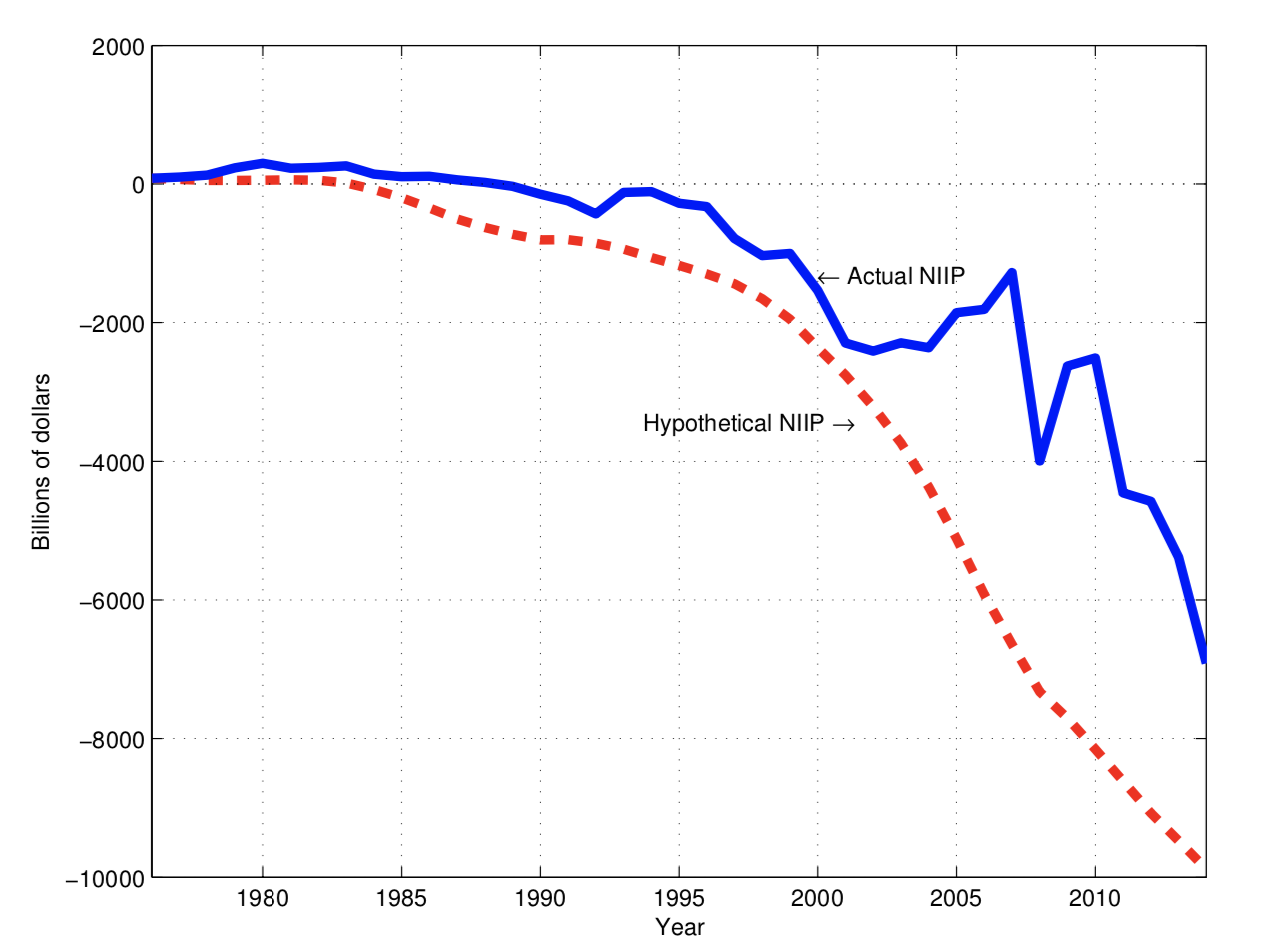
\includegraphics[width = 0.85\textwidth]{FIGURES/IIP_US.png}
  \end{figure}
  \vspace{-0.5cm}
  \begin{minipage}{\columnwidth}
  \footnotesize
  Source: Schmitt-Grohe, Uribe, Woodford, Fig. 1.6.
  \end{minipage}
\end{frame}

\section{Balance of Payments, IIP dynamics}
\begin{frame}
\frametitle{Outline}
\tableofcontents[currentsection]
\end{frame}

\begin{frame}{Model for Balance of Payments and IIP}
  We will assume a simplified structure for the analysis:
  \begin{mytemize}
  \item Trade Balance (TB, same as  PCA) can be computed from the GDP decomposition: $$TB_t = Y_t - C_t - I_t - G_t$$
	%Assume $Y_t$ exogenous and $I_t = G_t = 0$. Then, if $C_t$ is computed, $TB_t = Y_t - C_t$ follows automatically. 
  \item \tb{Income balance} -- financial income only. 
  Further, assume a sigle world interest rate $r_t$ for all assets and liabilities \rarr income balance is $r_t IPP_t$
\item Then, simple formula for CA: 
  \begin{align*}
  CA_t &= TB_t + r_t IPP_t \\ &= \underbrace{Y_t+ r_t IPP_t}_{\text{National Income}} - C_t - I_t - G_t 
  \end{align*}

  \end{mytemize}

\end{frame}

  \begin{frame}{Simplified dynamics of IPP}
	Simplified BOP identity is $CA_t = FA_t$ (no capital account, no errors and omissions)\\
	\vfill
	Replace in the IPP dynamics formula (without valuation changes): 
	  \begin{align*}
	  IIP_{t+1} &= IIP_t + CA_t \\
	  			&= IIP_t + TB_t + r_t IIP_t \\
	  &= (1+r_t) IIP_t + TB_t 
	  \end{align*}
  \end{frame}

  \begin{frame}{IIP and future trade balances}
	\vspace{-5cm}
	$$IIP_{t+1} = (1+r_t) IIP_t + TB_t $$
	Recursive relationship. Substitute $IPP_{t+1}$, then $IPP_{t+2}$ and so on. Result?
	

  \end{frame}

  \begin{frame}{IIP and future trade balances: interpretation}
	\begin{mytemize}
	  \item Assume $IIP_t<0$ -- country is a \textbf{net debtor} (not sovereign debt, but all sectors)
	  \item Then, country must run future \tb{trade surplus} on average (with more importance to surpluses that are in near future)
		\begin{mytemize}
		\item Otherwise, debts cannot be repaid
		\end{mytemize}
	  \item Assume $IIP_t>0$ -- country is a \textbf{net creditor} of rest of the world 
	  \item Then, country must run future \tb{trade deficits} on average (with more importance to deficits that are in near future)
		\begin{mytemize}
		\item Otherwise, debts of non-residents cannot be repaid
		\end{mytemize}
	\end{mytemize}
	\vfill
	\rarr Perpetual trade surpluses / trade deficits can be sustainable if very negative/very positive IIP to begin with. \textbf{$\{r_t\}$ matter, too}
  \end{frame}
\section{2-period Open Economy}
\begin{frame}
\frametitle{Outline}
\tableofcontents[currentsection]
\end{frame}

\begin{frame}{%
\protect\hypertarget{simple-two-period-economy}{%
Simple two-period economy}}
Recall a 2-period consumer problem (Lecture 5):
\begin{align*}
    \max_{C_1, C_2}  u(C_1) &+ \beta E u(C_2)  \\
    \text{s.t.} 
     C_1 +  \Omega_2  &= w_1 \bar L_1 + (1+r_1) \Omega_1  \\
     C_2 & =  w_2 \bar L_2  + (1+r_2) \Omega_2
  \end{align*}

An intertemporal budget constraint is obtained by eliminating
\(\Omega_2\):
\[C_1 + C_2/(1+ E r_2) = (1+r_1)\Omega_1 + w_1 \bar L_1 + w_2 \bar L_2/(1+E r_2)\]
and optimal consumption is obtained in a standard way. \vfill
Assume 
linear production \(Y_t = A_t L_t\); firms have no profits
\rarr \(w_t = A_t\). \\ Trade balance:
\(TB_t = A_t L_t - C_t\). \vfill 
Nowhere to invest in
the economy (no capital nor government) \rarr \(\Omega_t = IIP_t\).
Then, consumer savings \(\Omega_2 - \Omega_1 = IIP_2-IIP_1 = CA_1\).
\textit{[Verify it is true using period 1 budget constraint.]}

\end{frame}

\begin{frame}{%
\protect\hypertarget{productivity-shock-transitory-vs.permanent}{%
Productivity shock: temporary vs.~permanent}}

Assume a positive shock on period-1 productivity \(A_1\) \rarr GDP
rises, but desired consumption also rises. What is the net effect on
trade balance and current account?

\begin{mytemize}

\item
  In this economy, net effect always \textbf{positive}: recall that
  \(\Delta C_1 < \Delta Y_1\) because of consumption smoothing
  \rarr \(\Delta TB_1 = \Delta Y_1 - \Delta C_1 > 0\). Same effect for
  \(CA_1\) since \(CA_1 = TB_1 + r_1 \Omega_1\), with \(\Omega_1\)
  pre-determined
\item
  The effect on \(TB_2\) must be negative, since
  \(\Omega_1 = TB_1 + \frac{TB_2}{1+r_2}\) in a 2-period economy.
  Another proof: \(\Delta C_2 > 0\) because of consumption smoothing,
  but \(\Delta Y_2 = 0\).
\end{mytemize}
\vfill
Then, assume a \textbf{permanent shock}: both \(A_1\) and \(A_2\) rise.
What are effects on \(TB_1, CA_1\)?

\begin{mytemize}

\item
  Ambiguous: the shock allows for \(\Delta C_1 > 0, \Delta C_2 > 0\)
  with both \(\Delta C_1> \Delta Y_1\) and \(\Delta C_1< \Delta Y_1\).
\end{mytemize}

\end{frame}

\begin{frame}{%
\protect\hypertarget{terms-of-trade}{%
Terms of trade}}

Implicit assumption above: goods have same price
domestically and abroad. Assume domestic (exportable) goods price is \(P^X_t\)
 and foreign (importable) goods price is
\(P^M_t\).
\vfill
\tb{Terms of trade}:  \(TT_t = P^X_t/P^M_t\). Higher level
of terms of trade beneficial for the economy overall: it sells goods for
\(P^X_t\), buys goods for \(P^M_t\). \vfill \textbf{Assume all produced
goods exported, all consumed goods imported.} Budget constraints are
then:

\begin{align*}
     P^M_1 C_1 + P_1^M \Omega_2  &= P^X_1 w_1 \bar L_1 + (1+i_1) P_0^M \Omega_1  \\
     P^M_2 C_2 & =  P^X_2 w_2 L_2  + (1+i_2) P_1^M \Omega_2
  \end{align*} 
\end{frame}

\begin{frame}{Terms of trade}
\begin{align*}
     P^M_1 C_1 + P_1^M \Omega_2  &= P^X_1 w_1 \bar L_1 + (1+i_1) P_0^M \Omega_1  \\
     P^M_2 C_2 & =  P^X_2 w_2 L_2  + (1+i_2) P_1^M \Omega_2
  \end{align*} 
  Divide both sides by \(P_1^M\) and \(P_2^M\),
respectively, and use
\(1+r_t = (1+i_1)/(1+\pi_t) = (1+i_t)P^M_{t-1}/P^M_t\): \begin{align*}
     C_1 + \Omega_2  &= \textcolor{red}{TT_1} w_1 \bar L_1 + (1+r_1) \Omega_1  \\
     C_2 & =  \textcolor{red}{TT_2} w_2 L_2  + (1+r_2) \Omega_2
  \end{align*} \rarr \textbf{terms of trade shock has same effect as a
  productivity shock} (exported production and imported production assumptions are important)
\end{frame}

\begin{frame}{Production with capital}
  Consider capital in the same 2-period model.
  With fixed labor, the static firm problem is:

  $$\max_{K_t} A_t F(K_t, \bar L_t) - (1+r_{t})K_t + (1-\delta)K_t $$
  and the FOC is $A_t \frac{\partial F(K_t, \bar L_t)}{K_t} =  r_t + \delta$ \\
\vfill 
Under standard assumptions of $\frac{\partial F(K_t, \bar L_t)}{\partial K_t} >0, \frac{\partial^2 F(K_t, \bar L_t)}{(\partial K_t)^2}<0$: 

\begin{mynumerate}
\item  $K_t$ \textbf{depends negatively} on $r_t$ 
\item same for previous period's investment: $I_{t-1} = K_{t} - (1-\delta)K_{t-1}$ (where $K_{t-1}$ pre-determined)
\item $K_t$, $I_{t-1}$ \textbf{depend positively} on productivity $A_t$
\end{mynumerate}


\end{frame}

\end{document}
